%!TEX root=masterproef.tex

\section{Draadloze sensornetwerken}
\label{section:landscape}

``\emph{Waarom is het belangrijk om beveiliging van draadloze sensornetwerken
te bestuderen? Dit is toch al uitvoerig gedaan in andere vormen van
netwerken?}'' Op het eerste zicht is dit een zeer valabele vraag. Reeds sinds
de late jaren '80 kennen we concepten als \emph{firewalls} en virussen en
wormen. Meer dan 30 jaar reeds wordt er onderzoek gedaan naar
computerbeveiliging en solide oplossing zijn bedacht, uitgewerkt en
ge\"implementeerd. Wat houdt ons tegen om deze toe te passen op draadloze
sensornetwerken?

\subsection{Eigenschappen}

Ondanks het feit dat men knopen kan beschouwen als kleine computers en de
verbindingen die tussen hen tot stand komen een netwerk worden genoemd, eindigt
daar de vergelijking met andere bestaande technologie\"en volledig. Draadloze
sensoren en hun netwerken zijn een wereld op zich met zeer typerende
eigenschappen en eigen regels, mogelijkheden en beperkingen.

Een draadloze sensor is inderdaad een kleine computer, maar de nadruk ligt hier
op \emph{kleine}. De rekenkracht van een knoop is slechts een fractie van deze
van een hedendaagse computer en ligt in de tientallen megahertz, waar
hedendaagse systemen spreken in termen van gigahertz. De reden is evident:
draadloze sensornetwerken zijn volledig draadloos en worden ingezet in de meest
uiteenlopende, maar typisch afgelegen situaties. Ze zijn daarom gedurende lange
tijd afhankelijk van een zelfde batterijvoeding, en die moet dan ook optimaal
benut worden.

Ook het netwerk dat ze vormen vertoont typische eigenschappen die sterk
verschillen van de meer klassieke computernetwerken. Zo identificeert
\cite{blilat2012wireless} zes unieke eigenschappen van draadloze
sensornetwerken die leiden tot specifieke uitdagingen en opportuniteiten:

\begin{enumerate}

\item{De routing van de meeste draadloze sensornetwerken is
\emph{gestructureerd als een boom}. De concepten basisstation, router en knoop
werden eerder, samen met hun structuur, ge\"identificeerd in sectie
\ref{subsection:zigbee}.}

\item{De gegevens die door een knoop in het netwerk worden verzameld worden
typisch niet op zich beschouwd, maar \emph{geaggregeerd} met de metingen van
andere knopen. Dit wordt enerzijds gedaan om te compenseren voor effectieve
aberraties in de metingen zelf, maar ook om de onzekerheid van de
beschikbaarheid van de knopen te ondervangen.}

\item{Knopen zijn typisch de goedkope onderdelen van het netwerk en ze staan
slechts ten dienst van het eigenlijke doel van het netwerk, het verzamelen van
gegevens. Om die reden zijn ze eenvoudig vervangbaar en wordt dit als een
inherente eigenschap gezien. Het netwerk \emph{tolereert storingen} ten gevolge
van het wegvallen van knopen en vangt ze op door redundantie en aggregatie.}

\item{Om er voor te zorgen dat het netwerk zo min mogelijk belast wordt met het
verzenden van gegevens, worden meetgegevens zo dicht mogelijk bij de
oorspronkelijke knoop \emph{gefilterd en verwerkt}.}

\item{Een draadloos sensornetwerk bestaat uit knopen en niets anders. Elke
knoop is tegelijkertijd een \emph{sensor en router}, wat resulteert in een
optimalisatie van het netwerkverkeer.}

\item{De werking van een knoop kent een typisch \emph{gefaseerd zendpatroon}:
het verzamelen van meetgegevens, het ontvangen van gegevens van andere knoops en
het doorsturen van geaggregeerde gegevens naar hoger liggende knopen. Hierdoor
kan elke knoop zijn zender gedurende bepaalde periodes volledig afzetten,
natuurlijk om energie te besparen.}

\end{enumerate}

Dit beeld vinden we ook terug bij \cite{aschenbruck2012security} die de
situatie van draadloze sensornetwerken samenvat in drie zeer typische en
problematisch bronnen van beveiligingsproblemen: de beperkingen qua middelen en
dan vooral de energievoorziening, de fysieke toegankelijkheid die leidt tot de
mogelijkheid van het veroveren van knopen en de verwerking van gegevens die
reeds binnen het netwerk gebeurt, waardoor het bv. onmogelijkheid om encryptie
toe te passen tussen zender en ontvanger, waardoor tussenliggende verwerking
uitgesloten wordt.

\subsection{Inbraak detectie}

Maar ook het probleemgebied waarin draadloze sensornetwerken in deze thesis
vertoeven, maakt het op nog meer vlakken verschillend van meer een meer
klassieke computernetwerk setting.

In \cite{zhang2000intrusion} wordt een zeer algemene, maar zeer correcte
definitie gegeven van inbraak detectie.

\begin{quote}
\emph{Intrusion detection ... involves capturing audit data and reasoning about
the evidence in the data to determine whether the system is under attack.}
\end{quote}

Inbraakbeveiliging omvat twee essenti\"ele activiteiten: het vastleggen van
audit gegevens en het redeneren over deze gegevens. In het geval van draadloze
sensornetwerken moeten we het aspect \emph{systeem} op twee manieren
interpreteren: enerzijds als een knoop en anderzijds als het hele netwerk op
zich. Dit onderscheid bestaat ook in meer klassieke computernetwerken in de
vorm van \emph{systeem} en \emph{netwerk} inbraakdetectie.

In de context van draadloze sensornetwerken zal dit onderscheid zich echter
veel meer uitgesproken profileren omdat het netwerk hier geen centraal medium
is. Daar waar het netwerk in een klassieke opstelling typisch vanuit \'e\'en
systeem kon gecontroleerd worden door het afleiden van alle netwerkverkeer naar
\'e\'en enkele inbraakdetectie probe, is dit in het geval van een draadloos
sensornetwerk niet langer mogelijk. Het draadloze aspect maakt dat er geen
controleerbare toegangswegen meer zijn naar elke knoop en dat dus elke knoop
letterlijk op zichzelf aangewezen is.

Samen met het wegvallen van een centrale inbraakdetetie, valt ook de centrale
bescherming op netwerk niveau weg. Binnen een draaloos sensornetwerk is het ook
niet mogelijk om te genieten van de bescherming van een \emph{firewall}. Er is
niet langer een alles omringende bescherming, niet op logisch of netwerk vlak,
maar ook op fysisch vlak. Aangezien draadloze sensornetwerken typisch open en
blood in de buitenwereld ge\"installeerd worden, en dit voor langere periodes
zonder aanwezigheid van een eigenaar, kunnen ze ook fysiek benaderd worden door
ieder dat dat wil. Zelfs de elementaire zekerheid van een fysieke bescherming
in een bv. datacenter, komt bij draadloze sensornetwerken volledig te vervallen.

Zeer terecht stelt \cite{perrig2004security} daarom ook dat de eerste zorg
omtrent de beveiliging van draadloze sensor netwerken een veilige manier om de
groep van sensoren te beheren is. De manier waarop nieuwe knopen in het netwerk
worden opgenomen en de beveiliging van de onderlinge communicatie is van
primordiaal belang. Voorkomen is beter dan genezen.

Maar we moeten ook realistisch zijn. Geen door mensenhanden gemaakt systeem is
feilloos en nagenoeg elk ge\"informatiseerd system zal met de nodige inzet en
moeite veroverd kunnen worden. Op dat ogenblik is het belangrijk dat er een
tweede verdedigingslinie is: de inbraak detectie. In het geval van draadloze
sensornetwerken is dit dus misschien nog prangender, omdat er niet langer een
fysieke bescherming is, noch een centrale netwerkbescherming in de vorm van bv.
een \emph{firewall}.

\subsection{De tegenstander en zijn aanvallen}

Tijd om kennis te maken met onze tegenstander. Wat is zijn doel? Welke middelen
heeft hij ter beschikking? Hoe kunnen we zijn aanvallen identificeren?

\cite{aschenbruck2012security} identificeert vier fundamentele doelen die
nagestreefd worden door een aanvaller: het manipuleren van gegevens, het
afluisteren van communicatie, het weerhouden van gegevens en toegang verkrijgen
tot het netwerk. Dezelfde doelen vinden we ook bv. terug bij
\cite{blilat2012wireless}, zij het in een andere opdeling: het afluisteren van
communicatie, het analyseren, verstoren en kapen van netwerkverkeer en fysieke
aanvallen.

Aanvallen kunnen volgens \cite{dargie2010fundamentals} ingedeeld worden in vijf
klassen: aanvallen die het netwerk weerhouden om zijn diensten te realiseren
(\emph{Denial-of-Service} or \emph{DoS}), aanvallen op het niveau van de
routing binnen het netwerk, aanvallen gericht op de transport algoritmes binnen
het netwerk, aanvallen op het aggregerende karakter van het netwerk en
aanvallen gericht op de privacy van de deelnemers in de werking van het netwerk.

\cite{aschenbruck2012security} ervaart DoS eerder als een doel en deelt de
aanvallen vervolgens op in vier licht verschillende categorie\"en die correcter
aansluiten bij een draadloos sensornetwerk. Zo worden de volgende categorie\"en
aangegeven: het fysieke niveau waar een aanvaller gebruik maakt van middelen om
het alomtegenwoordig draadloos netwerk te benaderen, het niveau waarop het
fysieke niveau benaderd wordt door de knopen, de zgn. \emph{Medium-ACcess
layer} of \emph{MAC} laag, het niveau van de routing en het niveau van de knoop
als een functionele eenheid. Het is duidelijk dat er feitelijk een grote
tweeledigheid wordt gecreeerd tussen enerzijds het draadloze netwerk en
anderzijds de knoop op zich. Op elk van deze niveaus identificeert men
vervolgens typerende aanvallen.

\subsubsection*{Fysieke laag}

Sniffing

Jamming

\subsubsection*{MAC laag}

Rushing

Denial-of-Sleep

\TODO \cite{dargie2010fundamentals} identificeert ook nog Flooding 

\subsubsection*{Routing laag}

Sinkhole

Wormhole

Sybil

\subsubsection*{De knoop}

Verplaatsen van een knoop

Verwijderen van een knoop

Introductie van nieuwe knoop

Toegang tot het geheugen van een knoop

Herprogrammeren van een knoop

\TODO -> verdedigingen

Figuur \ref{fig:wsn-threat-analysis} visualiseert deze volledige
dreigingsanalyse.

\begin{figure}
  \centering
  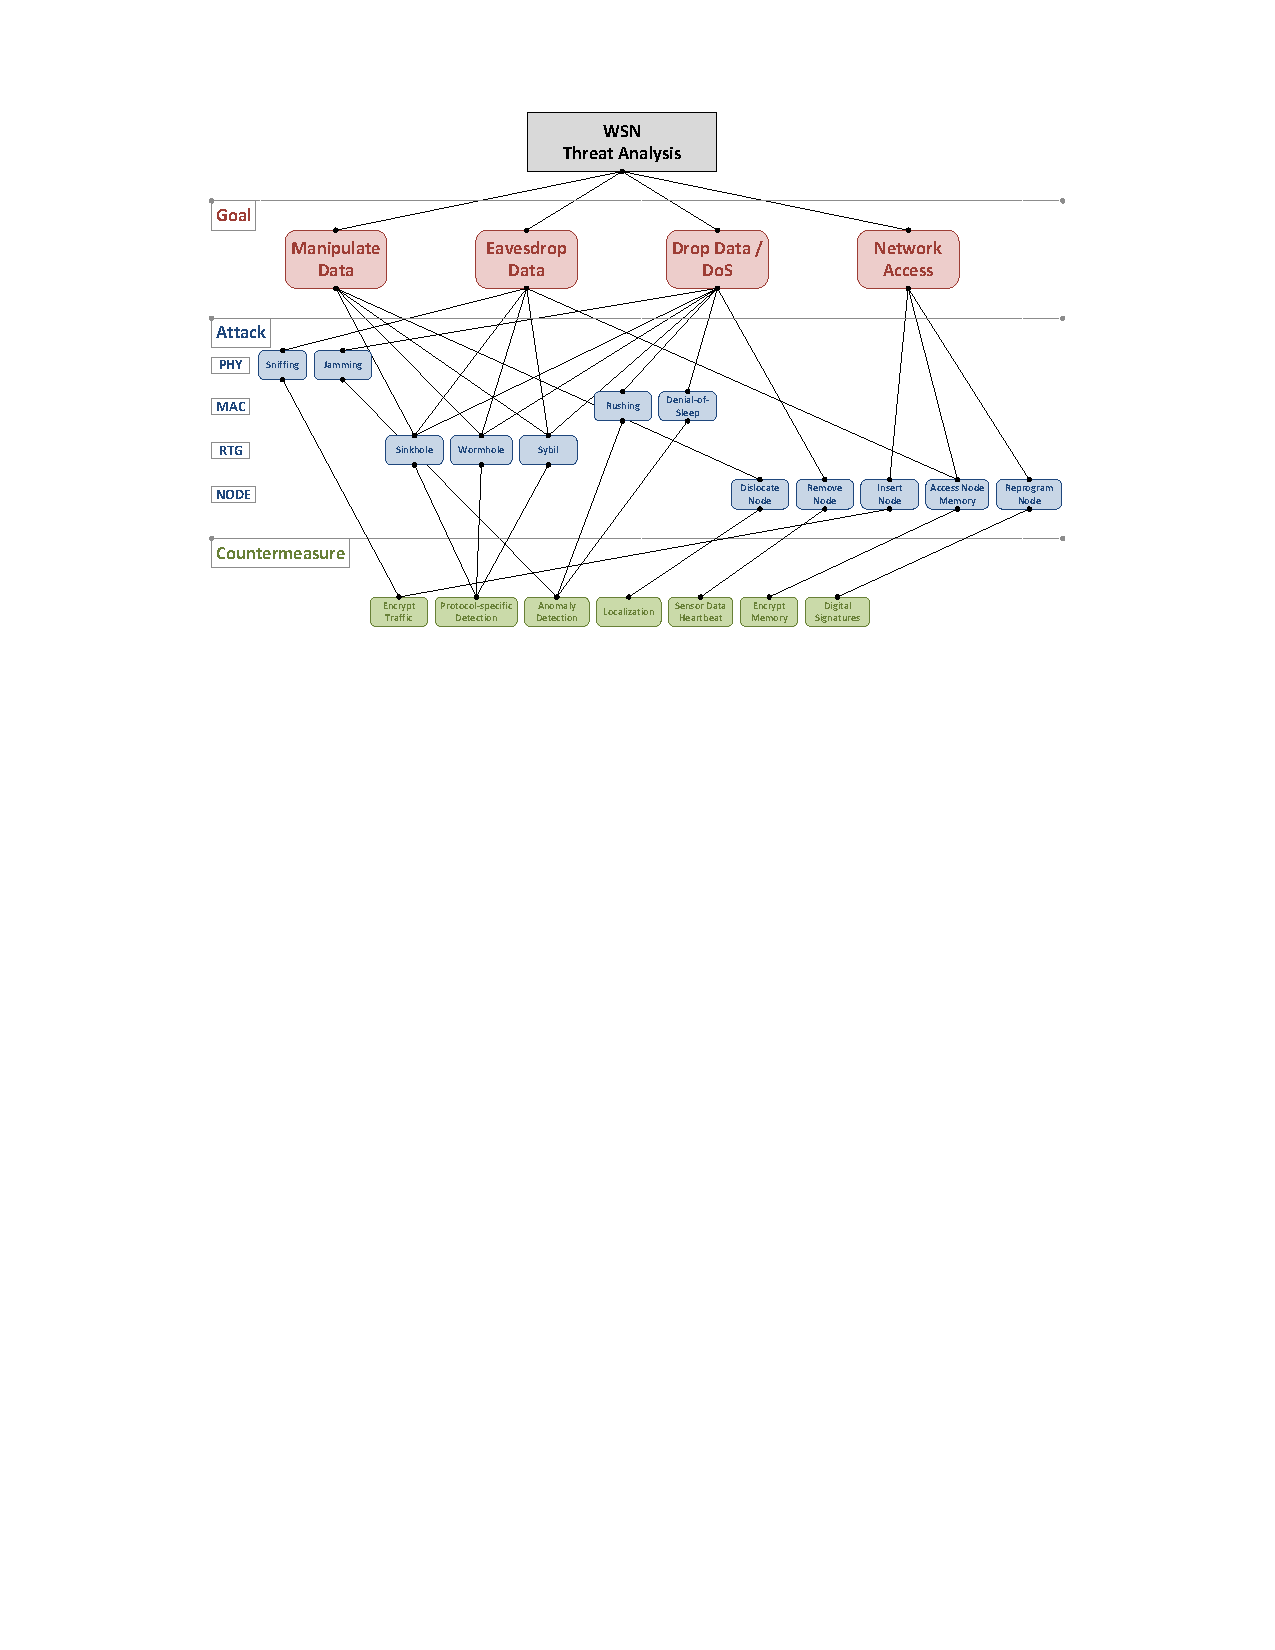
\includegraphics[width=0.9\linewidth]{resources/wsn-threat-analysis.pdf}
  \caption{Draadloze sensornetwerk dreigingsanalyse.}
  \label{fig:wsn-threat-analysis}
\end{figure}

\TODO -> verdediging ok, maar best ook opmerken, mocht verdediging falen

Identificatie van aanvallen wordt door \cite{zhang2000intrusion} gecatalogeerd
als \emph{misbruik} of \emph{anomalie}. Misbruik kan typisch gedetecteerd
worden aan de hand van patronen, terwijl voor het detecteren van anamolie\"en
er een patroon moet opgesteld worden en aberraties van dat patroon opgemerkt
moeten worden. Vooral dit laatste is typisch een delicaat aspect. Zo is het
onderscheid tussen een knoop die verplaatst werd en tijdelijk verkeerde routing
informatie verspreid en een knoop die veroverd werd en kwaadwillig foutieve
informatie uitstuurt, niet eenvoudig te maken.
